%%%%%%%%%%%%%%%%%%%%%%%%%%%%%%%%%%%%%%%%%%%%%%%%%%%%%%%%%%%%%%%%%%%%%%%%%%%%%%%%
%2345678901234567890123456789012345678901234567890123456789012345678901234567890
%        1         2         3         4         5         6         7         8

\documentclass[letterpaper, 10 pt, conference]{ieeeconf}  % Comment this line out if you need a4paper

%\documentclass[a4paper, 10pt, conference]{ieeeconf}      % Use this line for a4 paper

\IEEEoverridecommandlockouts                              % This command is only needed if 
                                                          % you want to use the \thanks command

\overrideIEEEmargins                                      % Needed to meet printer requirements.

% See the \addtolength command later in the file to balance the column lengths
% on the last page of the document

% The following packages can be found on http:\\www.ctan.org
%\usepackage{graphics} % for pdf, bitmapped graphics files
%\usepackage{epsfig} % for postscript graphics files
%\usepackage{mathptmx} % assumes new font selection scheme installed
%\usepackage{times} % assumes new font selection scheme installed
%\usepackage{amsmath} % assumes amsmath package installed
%\usepackage{amssymb}  % assumes amsmath package installed
\usepackage{graphicx}
\usepackage[export]{adjustbox}
\usepackage{hyperref}
\newcommand\tab[1][1cm]{\hspace*{#1}}
\graphicspath{ {images/} }


\title{\LARGE \bf
Self-driving robot with obstacle avoidance
}


\author{Pin-Wei Chen$^{1}$% <-this % stops a space
\thanks{*This work was supported by the Robotics Master Program in National Chiao Tung University, Taiwan}% <-this % stops a space
\thanks{$^{1}$Pin-Wei Chen, National Chiao Tung University, Taiwan.		{\tt\small ccpwearth@gmail.com}}%
}


\begin{document}

\maketitle
\thispagestyle{empty}
\pagestyle{empty}


\section{INTRODUCTION \& MOTIVATION}

The purpose of this project is to build a robot which can do self-driving task in an environment with obstacles, which is also the task in RobotX. I will try to give the robot a pair of latitude and longitude, and I will let the robot navigate to the goal point and also avoid the obstacles. And then I will test this system in marine Gazebo enviroment, and replace the wheel robot to WAM-V gazebo model.

\section{SYSTEM ARCHITECTURE \& EQUIPMENTS}

I use the wood and some Aluminum stick to build the robot. My robot has IMU, GPS, Wheel odometry and LIDAR (Velodyne VLP-16) on it as its' sensors.


\begin{figure}[h] % t means put this image at the top 
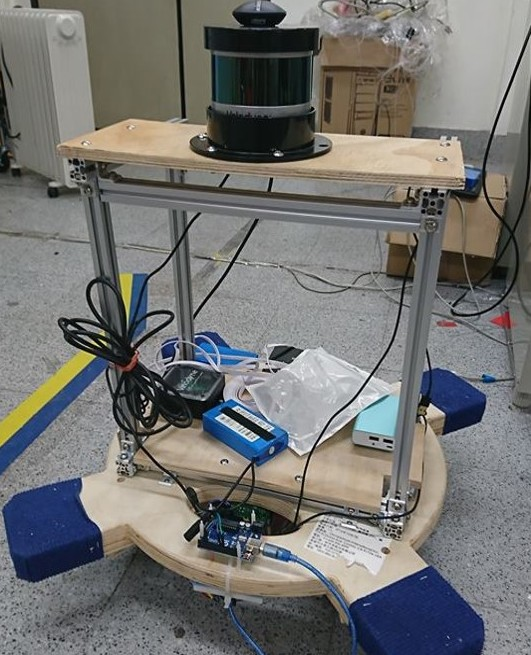
\includegraphics[width=0.8\columnwidth]{robot}
\centering
\caption{Self-driving robot}
\label{figure:robot}
\end{figure}

\begin{figure}[t] % h means put this image here
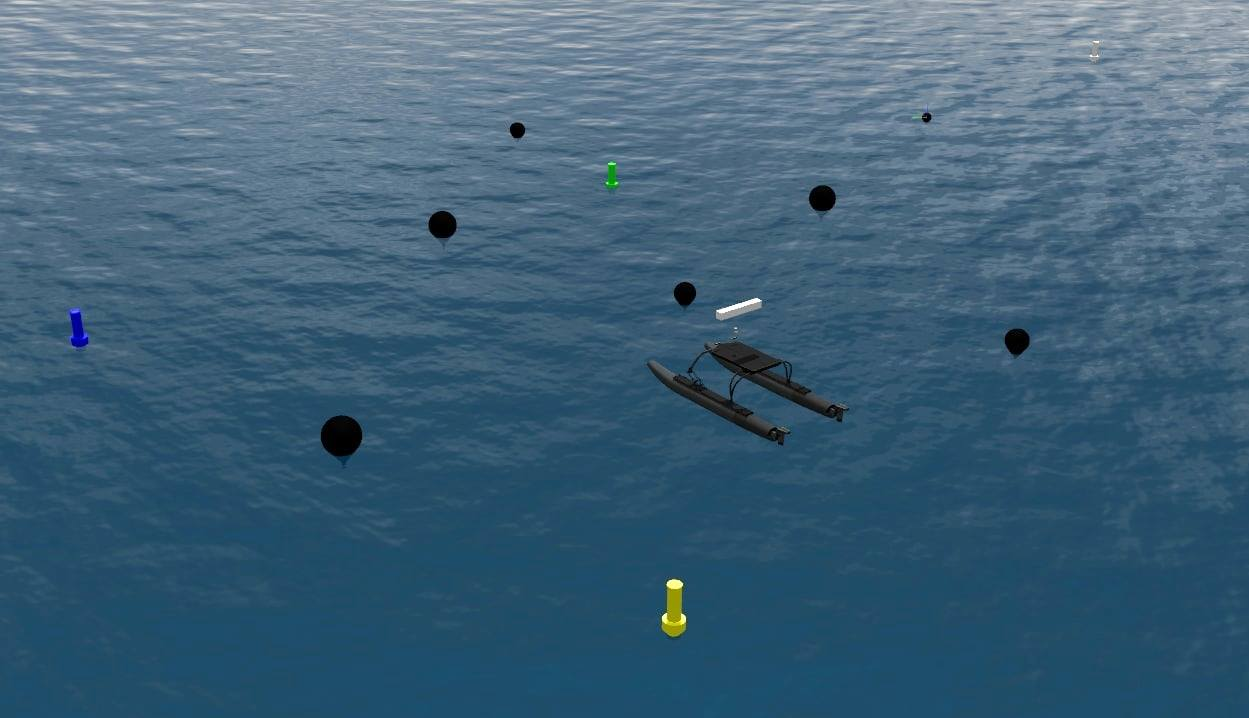
\includegraphics[width=0.9\columnwidth]{gazebo}
\centering
\caption{Gazebo WAM-V obstacle avoidance}
 \label{figure: WAM-V}
\end{figure}

\section{SPECIFIC AIMS}

\begin{itemize}
\item Localize robot with GPS, IMU, wheel odometry and LIDAR.
\end{itemize}

\begin{itemize}
\item Use point cloud to cluster and find the obstacle
\end{itemize}

\begin{itemize}
\item Plan a path to let the vehicle navigate without collision
\end{itemize}

\begin{itemize}
\item Build a simple global map to describe the obstacle position
\end{itemize}

\section{APPROACH}

\subsection{Localization}

I use IMU, GPS and wheel odometry to do EKF(Extended Kalman Filter). Also, I add LIDAR measurement to do SLAM (GMapping). And these two way can both get a robot odometry measurement. So I take these two odometry data do fusion again, and then I can get a very good robot localization and mapping.

\subsection{Point cloud Processing}

First, I make the noise filter, which can remove the outlier noise. And then I use plane filter to remove the floor, because the floor will affect our clustering result. Finally, I use K-means to do clustering, and then use a convex hull to present the obstacle by its' vertex. As a result, each obstacle can be present as a list of points.

\subsection{Path Planning and Following}

I choose a method refer from the paper~\cite{1527001} to do path planning, and use pure pursuit to follow the path. Then it can let the robot achieve goal point and also avoid obstacles.

\subsection{Demo videos} 
\begin{itemize}
\item Pure pursuit algorithm visualization: 
\end{itemize}
\tab\url{https://youtu.be/DdaZkm7_bjI}
\begin{itemize}
\item Self-driving at EE-building indoor: 
\end{itemize}
\tab\url{https://youtu.be/ve4Mln4D1xo}
\begin{itemize}
\item Self-driving at EE-building outdoor: 
\end{itemize}
\tab\url{https://youtu.be/E1anLPuXjxs}
\begin{itemize}
\item Self-driving WAM-V for RobotX task6: 
\end{itemize}
\tab\url{https://goo.gl/sDwa9j}

\addtolength{\textheight}{-12cm}   % This command serves to balance the column lengths
                                  % on the last page of the document manually. It shortens
                                  % the textheight of the last page by a suitable amount.
                                  % This command does not take effect until the next page
                                  % so it should come on the page before the last. Make
                                  % sure that you do not shorten the textheight too much.

\bibliographystyle{IEEEtran}
\bibliography{egbib}

\end{document}
